\chapter{定价与偏差解释}\label{research_method}
    \section{期权的定价模型}\label{pricing_model}
    本文首先采用Black-Scholes模型对比特币进行定价。Black-Scholes模型由Black和Scholes在1972年提出\cite{J-1972},根据其研究,Black-Scholes模型对交易资产及其市场有如下假设:
    \begin{itemize}
        \item 存在已知且恒定的无风险收益率r。
        \item 资产价格为带漂移随机游走过程, 即$dS={\mu}Sdt+{\sigma}SdW$,其中价格波动率$\sigma$为已知的常数。在这一假设下资产的收益率服从对数正态分布。
        \item 期权为欧式期权,即只有到期时期权的购买者才能够行权。
        \item 买卖期权和标的资产时不会产生交易费用和其他损失。
        \item 能够以无风险利率自由借入借出任意数量的资产。
        \item 对卖空操作无限制。
        \item 不存在无风险套利机会。
        \item 资产不支付红利。
    \end{itemize}
    在以上假设下,市场为有效且供给和需求达到均衡,故不存在套利空间。期权和股票构建的对冲组合应该只能获得无风险收益。根据对冲组合价值的现值,可以得到如下的期权定价公式:
    \begin{equation}\label{bs-call}
            C=S*N(d_1)-X*e^{-rT}*N(d_2) 
    \end{equation}
    \begin{equation}\label{bs-put}
        P=X*e^{-rT}*N(-d_2)-S*N(-d_1)
    \end{equation}
    其中
    \begin{equation*}
        \begin{split}
        d_1=\frac{ln(S/X)+(r+\sigma^2/2)T}{\sigma{\sqrt{T}}} \\
        d_2=\frac{ln(S/X)+(r-\sigma^2/2)T}{\sigma{\sqrt{T}}}
        \end{split}
    \end{equation*}
    C为看涨期权价格,P为看跌期权价格,S为标的资产价格,X为行权价格,r为无风险利率,T为距离到期日时间,$\sigma$为资产收益率的波动率。
    
    比起股票或其他传统金融资产,比特币市场更符合Black-Scholes模型的部分假设,这些假设更有利于进行推导模型时构建的delta-对冲过程:
        \begin{itemize}
            \item 比特币为连续交易,无假日和休市时间,可以在任意时间买卖。
            \item 比特币可以分割成(足够小的)任意单位买卖,而非必须整数。
        \end{itemize}
    
    \section{波动率的估计}\label{volatility-estimation}
    现实中,市场上的真实波动率并非恒定且已知的,因而无法直接采用\ref{bs-call}和\ref{bs-put}的公式对期权进行定价。可以采用多种方式对价格波动率进行估计,而真实价格与模型价格之间的差异部分也来自于不同投资者获得的波动率信息和对波动率的估计不同。
    投资者在市场上直接观察到的是近期一段时间比特币价格的波动。可以利用滚动窗口得到近期收益率的标准差估计,并将其作为期权到期日期前的期望波动率:
    \begin{equation}\label{volatility-rolling}
        \hat{\sigma}=\sum_{i=1}^{i=N}\frac{(r_{t-i}-\bar{r})^2}{N-1}
    \end{equation}
    其中$\bar{r}$为这一时期的平均收益率。本文中采用以一年(365天)为滚动窗口估计。用此方法得到的波动率估计相对稳定,同时也能反映出短期的波动趋势,数据期内估计波动率的变化如图\ref{fig:volatility}:
    \begin{figure}[H]
        \begin{small} 
            \begin{center}
                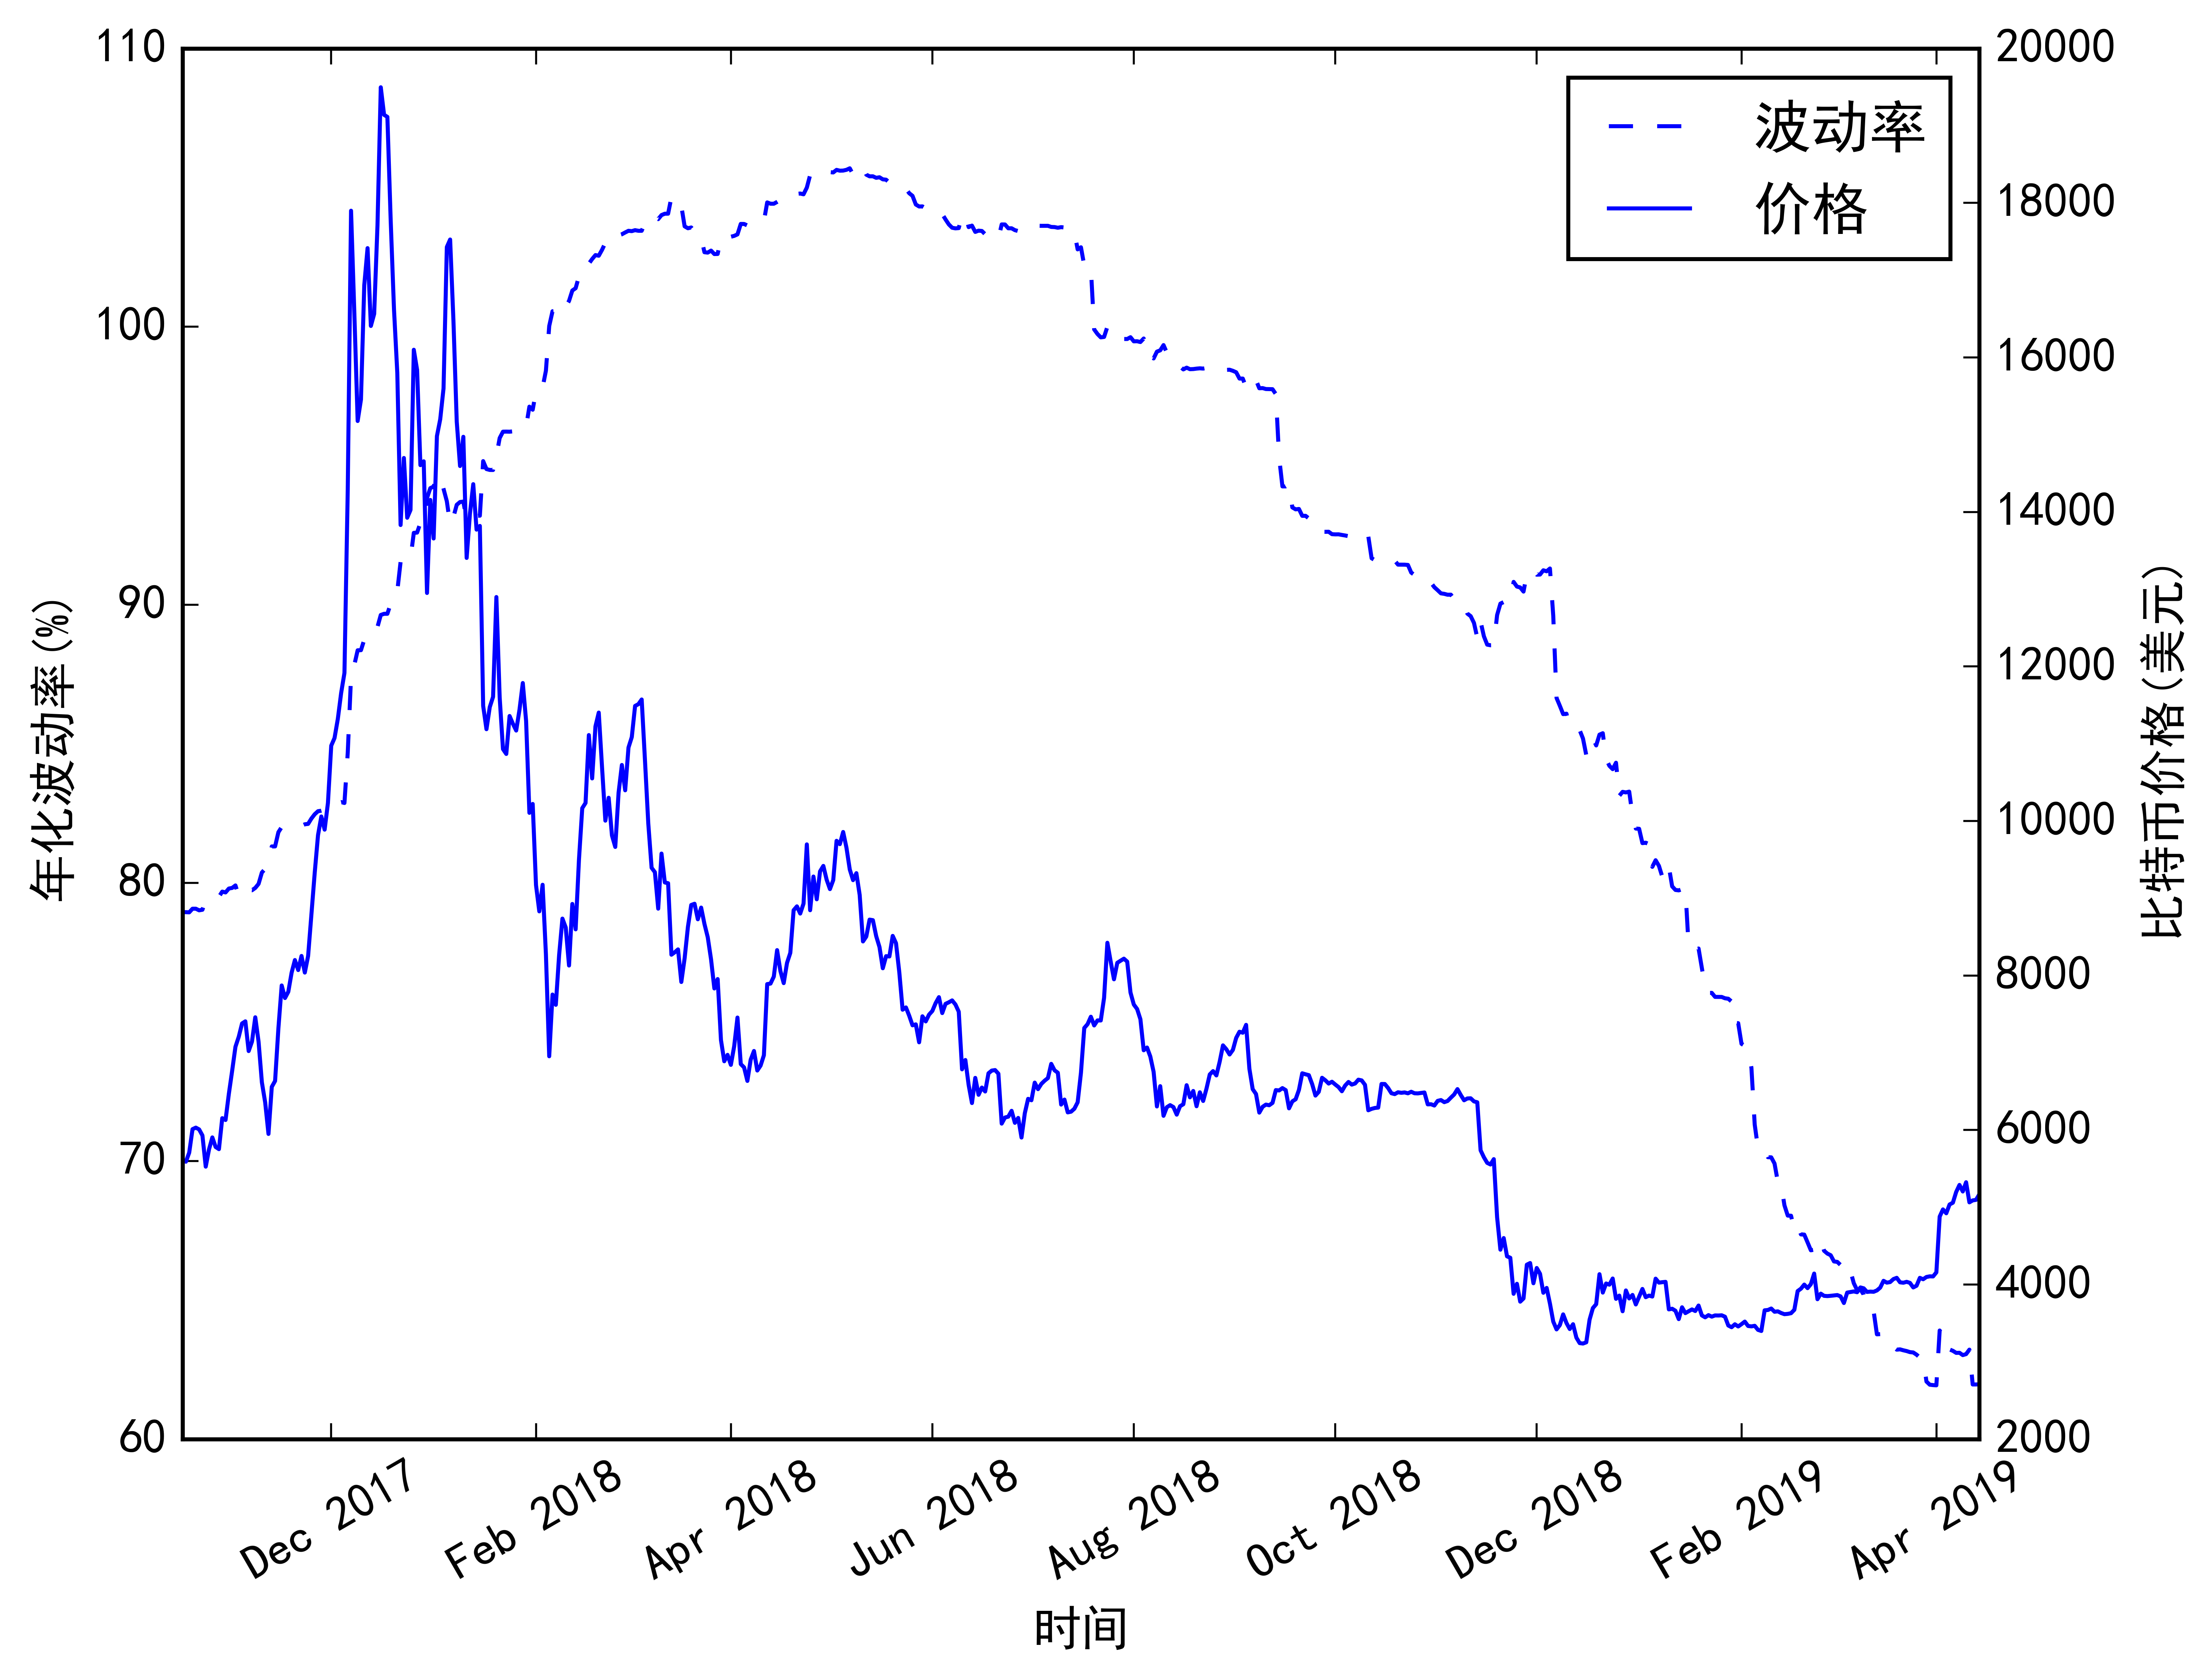
\includegraphics[width=0.95\textwidth]{figures/volatility.png}
            \end{center}
            \caption{数据期内比特币收益率滚动估计波动率与比特币价格}
            \label{fig:volatility}
        \end{small}
    \end{figure}
    这一估计充分捕捉到了2018年中的高波动率与18年末的低波动率,是目前比较好的对比特币收益波动的估计方式。从图中可以看到,比特币收益与波动率呈现一定的负相关,这也与股票市场上的情况较为类似。
    % \subsection{加权隐含波动率估计}
    % 从式\ref{bs-call}和\ref{bs-put}可以得出,期权的价格随波动率上升而上升。可以通过现在市场上的均衡期权价格得到一个$\sigma$的解,即为隐含波动率,这一预测方法利用了期权交易中的隐含信息。
    % 根据参考文献\cite{CHIRAS1978213},每日有多支期权且他们隐含波动率不同时,可以用以下公式获得当日的加权隐含波动率(WISD),该文献证明利用此方法得到的模型价格在股票市场上能得到极为显著的套利收益:
    % \begin{equation}
    %     WISD=\frac{\sum_{j=1}^{N}{ISD_j\frac{\partial{W_j}}{\partial{v_j}}\frac{v_j}{W_j}}}{\sum_{j=1}^{N}{\frac{\partial{W_j}}{\partial{v_j}}\frac{v_j}{W_j}}}
    % \end{equation}
    % 其中 , $WISD$为加权隐含波动率,$ISD_j$为第$j$个期权的隐含波动率,$N$为同一标的资产的期权个数,$\frac{\partial{W_j}}{\partial{v_j}}\frac{v_j}{W_j}$ 为期权价格相对于波动率的弹性。
    % \par{考虑到目前期权交易占整个比特币市场的交易比重并不大,故使用这一方式可能并不能有效反映期权定价中的波动率信息。同时部分日期比特币交易不够活跃,并不能得到准确的加权隐含波动率。}
    \section{定价结果}
按照第\ref{pricing_model}节的Black-Scholes模型\ref{bs-call}和\ref{bs-put},对每个期权的每条交易数据,将距离到期期限、数据期的波动率估计(采用第\ref{volatility-estimation}节的式\ref{volatility-rolling})、利率、当日比特币价格、行权价等信息输入模型,得到Black-Scholes模型定价。期权的真实价格为当天的成交量加权均价。在定价过程中,我们发现部分期权由于深度价外、而且期限较短,几乎没有模型价值,但仍有较高的真实价格,如果用二者数值的绝对差异将无法表现出这种定价差异的真实影响,相当于完全不包含模型的信息,故定义定价偏差为真实价格与模型价格之比:
\begin{equation}
    Price Diff=\frac{VWAP}{Model Price}
    \label{eq:diff}
\end{equation}


\par{保留共计600条记录。
600条记录的定价偏差的描述性统计以及按认购、认沽期权的分组统计之后结果如下:}
~\\
\begin{center}
    \begin{threeparttable}[H]
    
        \begin{small}
            \caption{定价偏差描述统计}
            \label{tab:option_bias_group}
                \begin{tabular}{lrrr}
\toprule
{} &    定价偏差 &  认购期权定价偏差 &  认沽期权定价偏差 \\
\midrule
count & 600.000 &   364.000 &   236.000 \\
mean  &   0.869 &     0.735 &     1.075 \\
std   &   0.526 &     0.289 &     0.711 \\
min   &   0.105 &     0.105 &     0.282 \\
25\%   &   0.614 &     0.537 &     0.739 \\
50\%   &   0.786 &     0.720 &     0.909 \\
75\%   &   0.997 &     0.886 &     1.162 \\
max   &   5.843 &     2.453 &     5.843 \\
\bottomrule
\end{tabular}

                
        \end{small} 
    \end{threeparttable}
\end{center}
~\\
\par{在合理的相对价值区间内,真实价格和模型价格差异仍然较大,最大接近6倍。最小接近十分之一,平均水平低于1,说明总体真实价格略低于模型价格。}
\par{分组统计结果中,认购期权的平均偏差低于1,而认沽期权的平均偏差高于1,且定价偏差最小值出现在认购期权、最大值出现在认沽期权,说明平均认购期权通常市场价格被低估,而认沽期权通常市场价格被高估。这是一种比较合理的现象:看跌期权在风险管理中提供了对下行风险的保护,同时也提供了做空比特币市场的重要工具。因而市场可能对看跌期权存在较高的需求。这也解释了为何总体的平均偏差低于1,因为认购期权的数量和交易数据条数都高于认沽期权。}
~\\
\par{为了初步展示定价偏差和期权价值程度之间的关系,我按照期权的相对价值(比特币价格/行权价)和期限分组,统计了各个组内定价偏差的平均值,以下是定价绝对偏差分组统计的结果:}
~\\
\begin{center}
\begin{threeparttable}[HT]
\centering
\caption{定价偏差分组统计}
\label{tab:option_bias_group}
\begin{small}

\begin{tabular}{lrrrrr}
\toprule
time\_cut &  0, 30 &  30, 60 &  60, 180 &  180, 624 &  mean \\
moneyness\_cut &          &           &            &             &       \\
\midrule
0.0, 0.6    &    1.027 &     1.126 &      1.075 &       1.129 & 1.109 \\
0.6, 0.9    &    0.822 &     0.968 &      0.911 &       1.029 & 0.937 \\
0.9, 1.1    &    0.812 &     0.774 &      0.953 &       1.102 & 0.843 \\
1.1, 3.9    &    1.010 &     1.054 &      1.016 &       1.185 & 1.063 \\
mean          &    0.856 &     0.903 &      0.961 &       1.098 &       \\
\bottomrule
\end{tabular}

\subcaption*{Panel A: 全部期权平均偏差}
\bigskip
\begin{tabular}{lrrrrr}
\toprule
time\_cut &  0, 30 &  30, 60 &  60, 180 &  180, 624 &  mean \\
moneyness\_cut &          &           &            &             &       \\
\midrule
0.0, 0.6    &          &     1.167 &      1.073 &       1.129 & 1.113 \\
0.6, 0.9    &    0.789 &     0.964 &      0.891 &       1.027 & 0.924 \\
0.9, 1.1    &    0.769 &     0.725 &      0.806 &       0.932 & 0.770 \\
1.1, 3.9    &    0.937 &     1.032 &      0.875 &       0.941 & 0.939 \\
mean          &    0.797 &     0.870 &      0.911 &       1.063 &       \\
\bottomrule
\end{tabular}

\caption*{Panel B: 认购期权平均偏差}
\bigskip
\begin{tabular}{lrrrrr}
\toprule
time\_cut &  0, 30 &  30, 60 &  60, 180 &  180, 624 &  mean \\
moneyness\_cut &          &           &            &             &       \\
\midrule
0.0, 0.6    &    1.027 &     1.003 &      1.104 &             & 1.042 \\
0.6, 0.9    &    0.981 &     1.011 &      1.137 &       1.045 & 1.035 \\
0.9, 1.1    &    0.880 &     0.924 &      1.155 &       1.303 & 0.975 \\
1.1, 3.9    &    1.058 &     1.058 &      1.051 &       1.302 & 1.115 \\
mean          &    0.951 &     0.997 &      1.107 &       1.234 &       \\
\bottomrule
\end{tabular}

\caption*{Panel C: 认沽期权平均偏差}
\begin{tablenotes}
    \footnotesize
    \item 注:money\_cut指期权价值程度分组边界(比特币价格/行权价),time\_cut指距到期期限分组边界(天)。因认购期权缺乏价值程度在0-0.6之间的,认沽期权缺乏期限大于180天的,故部分数据位置缺失。
\end{tablenotes}
        \end{small}
    \end{threeparttable}
        
\end{center}
~\\
\par{可以看到,总体上定价偏差随期限的上升呈一定增长趋势。从分不同方向结果直观而言,对于全部认沽期权,实值期权的偏差要小于虚值期权,同时整体上倾向于在值期权(即moneyness非常接近1)拥有最小的平均偏差,这符合期权常见的“波动率微笑”现象,即在值期权具有相对较小的隐含波动率(意味着相对较低的期权价格),而对于认购期权这一现象并不明显。}
\par{
    还有值得注意的现象是,随着期权期限的增长,低价值程度和高价值程度之间定价偏差的差异在逐渐缩小。即随着时间的增长,比特币未来价格的不确定性也在增长,故当前价值程度对于期权价格的影响开始减弱。
}
\section{隐含波动率}
隐含波动率即使得Black-Scholes模型价格等于真实价格的波动率参数,这一数值表示了隐含于期权市场价格中与波动率有关的信息。以期权相对价值(S/K)将全部期权分为五组,并求各组平均隐含波动率,以各组相对价值中位数为横轴,隐含波动率为纵轴绘制折线图如下:
\begin{figure}[H]
    \begin{small}
        \begin{center}
            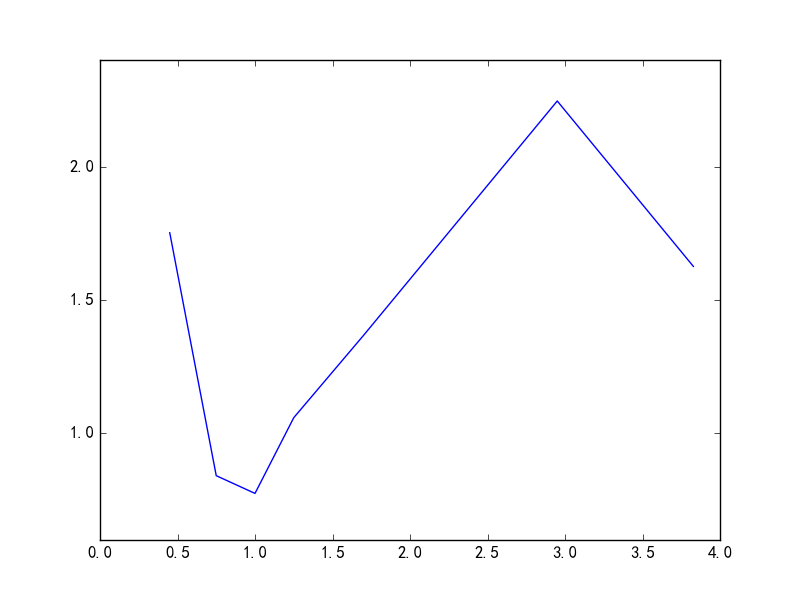
\includegraphics[width=0.95\textwidth]{figures/mean_isd.png}
        \end{center}
        \caption{隐含波动率分组曲线}
        \label{fig:mean_isd}
    \end{small}
\end{figure}
图像呈现出一定的“波动率微笑”性质,相对价值接近1的时候隐含波动率水平更低。本质上隐含波动率微笑现象反映了收益分布与对数正态分布之间的差异。
% \par{
%     波动率溢价:定义为从现在至期权到期日期间比特币波动率与期权隐含波动率之差。由于波动率越大,一般期权的价格越高,这一指标衡量了期权交易者对波动率的预测与未来期权波动率符合程度。
% }

    \section{对定价偏差的解释}\label{reg vars}
    波动率微笑现象反映出了期权的隐含波动率和其价值程度(即资产价格与行权价之比)存在规律性的关系,同理我们可以探究很多变量对于期权真实价格与模型价格之间偏差的系统性影响。通过构建回归模型并对变量的系数进行分析,我们可以识别不同因素对真实价格偏离部分的影响的方向,并对其做出解释。这些变量主要分为两个方面:比特币市场因素和期权因素。
    \subsection{比特币市场有关变量}
    \begin{itemize}
        \item log\_ret 比特币市场对数收益率
        \item volatility 比特币历史波动率
        \item skewness 比特币收益率历史偏度
        \item kurtosis 比特币收益率历史峰度
        \item amihud Amihud非流动性指标
        \item btc\_volume 比特币市场总交易量
        \item maxmin\_ratio 当日比特币交易所中价格最高者和最低者之比
    \end{itemize}
    
    这些指标衡量了比特币市场的市场环境。如波动率、偏度、峰度反映了投资者所处的风险情况,同时也属于识别出的模型设定问题,偏度和峰度的存在影响了而非流动性指标和maxmin\_ratio体现了市场的流动性情况,这些都可能造成真实价格同模型价格之间的偏差。maxmin\_ratio还能体现出比特币价格发现的完善程度,与利用期权套利的可行性有关。
    \subsection{期权自身有关变量}
    \begin{itemize}
        \item delta 期权根据Black-Scholes模型计算出的delta
        \item time 期权距离到期日的时间
        \item vol\_pre 期权的波动率溢价(Volatility Premimum),利用该期权当时的隐含波动率与当天至到期日之间的实现波动率之差计量。
        \item volume 期权当天交易量                                     
        
        \item open\_interest 期权当天公开的持仓量
        \item contract\_is\_call 哑变量,是否为认购期权,1为认购期权,0为认沽期权。 
    \end{itemize}
    这些指标能够衡量期权自身性质对真实价格的影响,主要是不同性质的期权可能导致投资者对其供给和需求的不平衡会造成期权价格的偏离。

    
\section{回归结果}
我们首先构建第\ref{reg vars}节提出的变量,并对其进行描述性统计。由于部分期权的交易价格不在期权价格的合理范围内,故无法用数值方法求得隐含波动率,将这部分数据删去后剩余577条数据。变量的描述统计和相关性矩阵如下:
\newpage
\newgeometry{top=1cm,bottom=1cm
}
\begin{landscape} 
    \begin{table}[H]
        \caption{解释变量的描述性统计}
        \resizebox{\linewidth}{!}{
        \begin{tabular}{lrrrrrrrrrrrrrrrrr}
\toprule
{} &  log\_ret &  volatility &  skewness &  amihud &  maxmin\_ratio &  btc\_volume &   time &  const\_delta\_5 &  vol\_pre &  spread &  open\_interest &  slope &  volume &  contract\_is\_call &  inter\_call\_money &  inter\_put\_money &  inter\_call\_skewness \\
\midrule
count &   577.00 &      577.00 &    577.00 &  577.00 &        577.00 &      577.00 & 577.00 &         577.00 &   577.00 &  577.00 &         577.00 & 577.00 &  577.00 &            577.00 &            577.00 &           577.00 &               577.00 \\
mean  &    -0.00 &        0.04 &     -0.39 &    0.04 &          1.04 &       22.45 &   3.75 &           0.14 &     0.01 &  272.88 &          62.84 &   0.00 &   19.48 &              0.60 &              0.58 &             0.41 &                -0.24 \\
std   &     0.05 &        0.02 &      0.76 &    0.02 &          0.03 &        0.40 &   1.00 &           0.47 &     0.02 &  430.01 &          99.58 &   0.00 &   29.35 &              0.49 &              0.50 &             0.51 &                 0.61 \\
min   &    -0.17 &        0.01 &     -4.50 &    0.01 &          1.00 &       21.30 &   2.08 &          -1.00 &    -0.06 & -225.00 &           0.00 &  -0.00 &    2.00 &              0.00 &              0.00 &             0.00 &                -4.50 \\
25\%   &    -0.03 &        0.03 &     -0.81 &    0.03 &          1.01 &       22.16 &   3.09 &          -0.31 &    -0.00 &  121.50 &           9.00 &  -0.00 &    3.00 &              0.00 &              0.00 &             0.00 &                -0.40 \\
50\%   &     0.00 &        0.04 &     -0.23 &    0.04 &          1.03 &       22.36 &   3.56 &           0.36 &     0.01 &  174.00 &          31.00 &   0.00 &    7.00 &              1.00 &              0.86 &             0.00 &                -0.00 \\
75\%   &     0.02 &        0.05 &      0.03 &    0.05 &          1.05 &       22.65 &   4.39 &           0.53 &     0.02 &  310.75 &          98.00 &   0.00 &   20.00 &              1.00 &              0.95 &             0.98 &                 0.00 \\
max   &     0.23 &        0.09 &      1.15 &    0.09 &          1.19 &       23.89 &   6.36 &           1.00 &     0.11 & 9000.00 &        1109.00 &   0.00 &  226.00 &              1.00 &              3.83 &             1.25 &                 1.03 \\
\bottomrule
\end{tabular}

        }
    \end{table}
    \begin{table}[H]
        \caption{解释变量的相关性矩阵}
        \resizebox{\linewidth}{!}{\begin{tabular}{lrrrrrrrrrrrrrrrrr}
\toprule
{} &  log\_ret &  volatility &  skewness &  amihud &  maxmin\_ratio &  btc\_volume &  time &  delta\_5 &  vol\_pre &  spread &  open\_interest &  slope &  volume &  contract\_is\_call &  inter\_call\_money &  inter\_put\_money &  inter\_call\_skewness \\
\midrule
log\_ret             &     1.00 &        0.02 &      0.13 &    0.03 &         -0.12 &       -0.01 &  0.05 &     0.09 &    -0.14 &   -0.02 &          -0.01 &   0.06 &   -0.02 &              0.03 &              0.05 &            -0.00 &                 0.08 \\
volatility          &     0.02 &        1.00 &      0.29 &    0.98 &          0.64 &        0.75 &  0.20 &     0.08 &     0.27 &    0.35 &          -0.20 &   0.07 &   -0.14 &             -0.13 &             -0.11 &             0.14 &                 0.23 \\
skewness            &     0.13 &        0.29 &      1.00 &    0.35 &          0.07 &        0.17 &  0.10 &     0.10 &     0.15 &    0.13 &           0.03 &   0.03 &   -0.06 &              0.01 &              0.05 &             0.00 &                 0.80 \\
amihud              &     0.03 &        0.98 &      0.35 &    1.00 &          0.61 &        0.71 &  0.19 &     0.08 &     0.27 &    0.33 &          -0.20 &   0.07 &   -0.15 &             -0.14 &             -0.11 &             0.15 &                 0.29 \\
maxmin\_ratio        &    -0.12 &        0.64 &      0.07 &    0.61 &          1.00 &        0.64 &  0.15 &     0.06 &    -0.02 &    0.35 &          -0.21 &   0.06 &   -0.13 &             -0.10 &             -0.04 &             0.10 &                 0.07 \\
btc\_volume          &    -0.01 &        0.75 &      0.17 &    0.71 &          0.64 &        1.00 &  0.14 &     0.09 &     0.17 &    0.36 &          -0.17 &   0.10 &   -0.10 &             -0.09 &             -0.03 &             0.10 &                 0.14 \\
time                &     0.05 &        0.20 &      0.10 &    0.19 &          0.15 &        0.14 &  1.00 &     0.17 &     0.21 &    0.32 &           0.02 &  -0.08 &   -0.02 &              0.15 &             -0.08 &            -0.12 &                 0.01 \\
delta\_5             &     0.09 &        0.08 &      0.10 &    0.08 &          0.06 &        0.09 &  0.17 &     1.00 &    -0.15 &    0.16 &          -0.00 &  -0.08 &    0.03 &              0.81 &              0.85 &            -0.73 &                -0.13 \\
vol\_pre             &    -0.14 &        0.27 &      0.15 &    0.27 &         -0.02 &        0.17 &  0.21 &    -0.15 &     1.00 &    0.20 &           0.07 &  -0.05 &   -0.02 &             -0.12 &             -0.18 &             0.10 &                 0.13 \\
spread              &    -0.02 &        0.35 &      0.13 &    0.33 &          0.35 &        0.36 &  0.32 &     0.16 &     0.20 &    1.00 &          -0.10 &   0.02 &   -0.08 &              0.02 &              0.20 &            -0.03 &                 0.10 \\
open\_interest       &    -0.01 &       -0.20 &      0.03 &   -0.20 &         -0.21 &       -0.17 &  0.02 &    -0.00 &     0.07 &   -0.10 &           1.00 &  -0.13 &    0.37 &              0.21 &              0.07 &            -0.20 &                -0.01 \\
slope               &     0.06 &        0.07 &      0.03 &    0.07 &          0.06 &        0.10 & -0.08 &    -0.08 &    -0.05 &    0.02 &          -0.13 &   1.00 &   -0.08 &             -0.42 &             -0.30 &             0.48 &                 0.16 \\
volume              &    -0.02 &       -0.14 &     -0.06 &   -0.15 &         -0.13 &       -0.10 & -0.02 &     0.03 &    -0.02 &   -0.08 &           0.37 &  -0.08 &    1.00 &              0.13 &              0.08 &            -0.12 &                -0.09 \\
contract\_is\_call    &     0.03 &       -0.13 &      0.01 &   -0.14 &         -0.10 &       -0.09 &  0.15 &     0.81 &    -0.12 &    0.02 &           0.21 &  -0.42 &    0.13 &              1.00 &              0.85 &            -0.97 &                -0.28 \\
inter\_call\_money    &     0.05 &       -0.11 &      0.05 &   -0.11 &         -0.04 &       -0.03 & -0.08 &     0.85 &    -0.18 &    0.20 &           0.07 &  -0.30 &    0.08 &              0.85 &              1.00 &            -0.82 &                -0.19 \\
inter\_put\_money     &    -0.00 &        0.14 &      0.00 &    0.15 &          0.10 &        0.10 & -0.12 &    -0.73 &     0.10 &   -0.03 &          -0.20 &   0.48 &   -0.12 &             -0.97 &             -0.82 &             1.00 &                 0.27 \\
inter\_call\_skewness &     0.08 &        0.23 &      0.80 &    0.29 &          0.07 &        0.14 &  0.01 &    -0.13 &     0.13 &    0.10 &          -0.01 &   0.16 &   -0.09 &             -0.28 &             -0.19 &             0.27 &                 1.00 \\
\bottomrule
\end{tabular}
    }
    \end{table}    
\end{landscape}

    \newpage
\restoregeometry
其中,log\_ret为当日比特币对数收益率、volatility为30天滚动估计收益波动率、skewness为30天滚动估计收益偏度、amihud为Amihud非流动性指标,maxmin\_ratio为交易所价格最大者与最小者之比,btc\_volume为当日比特币交易量,time为期权期限,delta\_5为当前模型下计算出的delta,
vol\_pre为波动率溢价(参见\ref{reg vars}),open\_interest为当日该期权持仓量,contract\_is\_call为指示变量,指期权是否为认购期权。
\par{其中,相对价值(比特币价格/行权价)的意义与期权的种类有关,对于认购期权,这一指标越高证明期权价值程度越深,对于认沽期权则完全相反,故构建两个交互变量inter\_call\_money和inter\_put\_money来表示不同类期权中的相对价值对定价偏差的影响。}
\par{从相关性矩阵可见,部分变量之间的相关性水平较高。可利用后向逐步回归的方法剔除部分变量,即先采用全部变量进行回归,再通过AIC信息熵损失最小法逐步选择去掉的变量并进行回归。最终,结合相关性矩阵并参考后向逐步回归结果,可以剔除掉比特币波动率、偏度、期权种类指示变量和偏度的交互项这几个变量。以偏差为解释变量,进行最小二乘法回归。为了验证结论的稳健性,我采用三种不同的数据集进行回归,包括了放宽现有准则和现有准则之外的数据。数据集说明和结果见下表:}
\newpage
\newgeometry{top=1cm}
\begin{center}
    \begin{threeparttable}[H]

        \caption{回归估计结果}
        \label{reg_table}
        \begin{tabular}{lccc}
\hline
                   & call$>$0.8,put<1.25 & call<0.8,put$>$1.25 & call$>$0.7,put<1.3  \\
\midrule
\midrule
Intercept          & -4.9902***          & 126234.9392         & -8.9433***          \\
                   & (1.1780)            & (281176.8611)       & (1.6272)            \\
log\_ret           & 0.5375*             & 96675.3767*         & 1.1359***           \\
                   & (0.3157)            & (57632.2696)        & (0.4335)            \\
kurtosis           & 0.1782***           & 6343.4584           & 0.2334***           \\
                   & (0.0281)            & (8426.4641)         & (0.0402)            \\
amihud             & 3.9838***           & -513881.4714*       & 1.6044              \\
                   & (1.2172)            & (271117.2178)       & (1.6661)            \\
maxmin\_ratio      & 1.0957              & 234087.8525*        & 3.5056***           \\
                   & (0.7814)            & (137447.4289)       & (1.0928)            \\
btc\_volume        & 0.2021***           & -15053.7342         & 0.2505***           \\
                   & (0.0577)            & (12875.2874)        & (0.0803)            \\
delta              & 0.4704***           & 73920.6879**        & 0.3092              \\
                   & (0.1492)            & (28877.8010)        & (0.1892)            \\
vol\_pre           & 12.5519***          & 1259228.9564***     & 16.8868***          \\
                   & (0.8931)            & (296926.5120)       & (1.2527)            \\
open\_interest     & -0.0000             & -12.0211            & -0.0001             \\
                   & (0.0001)            & (14.9864)           & (0.0002)            \\
time               & -0.1034***          & -14563.4822***      & -0.1560***          \\
                   & (0.0163)            & (4098.7171)         & (0.0230)            \\
contract\_is\_call & 0.0361              & 31960.2562          & 0.8275**            \\
                   & (0.2928)            & (37641.4193)        & (0.3676)            \\
inter\_call\_money & -0.4167***          & -37702.8170         & -0.5799***          \\
                   & (0.1124)            & (50739.3725)        & (0.1592)            \\
inter\_put\_money  & 0.2441              & 17446.6537          & 0.7069**            \\
                   & (0.2168)            & (12040.3093)        & (0.2900)            \\
observations       & 577.0000            & 354.0000            & 687.0000            \\
R-Squared          & 0.6242              & 0.1397              & 0.5286              \\
Adjusted R-Squared & 0.6162              & 0.1094              & 0.5202              \\
\hline
\end{tabular}
        
        \begin{tablenotes}
            \footnotesize
            \item *:p值<0.1, **:p值<0.05, ***:p值<0.01
            \item 括号中汇报估计系数的标准差。
            \item “call>0.8,put<1.25”指根据期权moneyness保留数据的阈值。第二列指认购moneyness小于0.8,认沽moneyness>1.25;第三列指认购moneyness大于0.7,认沽moneyness<1.3
            \item log\_ret:比特币对数收益率;kurtosis:比特币收益率峰度;amihud:amihud非流动性指标;maxmin\_ratio:比特币价格最大最小值比率;btc\_volume:当日交易量(取对数处理);delta:期权delta值;vol\_pre:期权波动率溢价;open\_interest:期权持仓量;time:期权期限;contract\_is\_call:期权是否为看涨期权;inter\_call\_money:期权是否为认购期权与moneyness交互项;inter\_put\_money:期权是否为认沽期权与moneyness交互项
        \end{tablenotes}
    \end{threeparttable}
\end{center}
\newpage
\restoregeometry
\par{三个不同范围样本的回归结果中,系数的显著性和正负方向均比较接近,其中第二列数据包含了前述过多的较大差异的数据点(即模型价格过小),故系数较大。同时,模型的R方在第二列数据和第三列数据中有明显的降低,表明当期权价值为明显的虚值时,其真实价格的偏离可能受到更多异质性因素或尚未考虑的因素影响。}
\par{
实际上,这里的定价差异相当于是假设B-S模型价格为供需平衡状态下的均衡价格,而偏差衡量了期权的供需不均衡的程度。一部分解释变量的系统性影响可以用供需来解释。峰度为比特币的收益分布与对数正态分布不符的衡量,其系数显著为正,证明了过高的尾部风险会推高期权的价格。比特币的交易量和收益衡量了短期市场的热度,当市场投资情绪较高时,对对冲的要求也更高,故此时对期权的需求更大,提升了期权的价格。}
\par{衡量比特币交易流动性的Amihud指标、最大价格与最小价格之比两个变量均与比特币市场的流动性有负相关关系,而在回归结果中对期权定价的相对偏差有显著正向关系。说明很可能随着比特币市场流动性下降,B-S模型推导过程中用到的delta-对冲模式不能完整实现,也就是利用期权进行套利的可行性降低。故而导致价格不能回到有效情况下的水准。
}
\par{对于和期权自身性质有关的变量,其中比较显著的影响是波动率溢价。波动率溢价变量本身用到了未来波动率信息,部分价格看上去过高的期权交易可以被认为是投资者获得了对于未来波动率会更高的信息,投资者自身对未来波动率的预测是影响期权供需的重要因素。delta对期权的市场价格也有高估的作用,delta本身度量了期权的“股性”,也就是期权价格随比特币价格变化的同步性,这可能说明市场上对期权的投机需求较高。除此之外,在控制其他变量不变的情况下,看涨期权价格会相对偏离更高,时间较长的反而导致真实价格相对偏低,与之前分组统计结果不符。一个可能的解释是看涨期权更容易受到其他变量的影响,导致其综合影响为期权的总体价格偏低。对于期权价值程度的交互变量而言,对于两种期权都是实值程度越深,定价偏差越小,这也符合股票市场上观察到的结果。期权的持仓量对整个模型几乎无影响,说明期权的流动性可能对价格偏差的影响不大\footnote{此处受数据限制,缺乏构建更有效的变量来证明}。整个模型的R方达到60$\%$以上,有一定的解释能力。}
\par{为了识别除了价值程度之外,其他变量是否在不同种类的期权中有不同的作用,同时是否有一些变量拉低了看涨期权的实际价格,将两种期权分组之后分别做最小二乘法回归(此处只采用表\ref{reg_table}第一列的数据集),结果如下:}
\newpage
\newgeometry{top=3cm}
\begin{center}
    \begin{threeparttable}[H]

        \caption{回归估计结果}

        \begin{tabular}{lcc}
\hline
                   &   �Ϲ���Ȩƫ��   &    �Ϲ���Ȩƫ��    \\
\midrule
\midrule
Intercept          & -1.7605*   & -17.8168***  \\
                   & (0.9617)   & (2.9802)     \\
log\_ret           & -1.4445*** & 2.7104***    \\
                   & (0.2854)   & (0.7118)     \\
amihud             & 10.0761*** & 6.2093**     \\
                   & (1.0310)   & (2.9473)     \\
maxmin\_ratio      & 0.2213     & 4.3309***    \\
                   & (0.6263)   & (1.6215)     \\
btc\_volume        & 0.0850*    & 0.6400***    \\
                   & (0.0484)   & (0.1451)     \\
const\_delta\_5    & 0.0966     & 0.6517***    \\
                   & (0.0766)   & (0.2016)     \\
vol\_pre           & 6.1960***  & 8.7675***    \\
                   & (0.8137)   & (2.5295)     \\
spread             & -0.0000    & -0.0003      \\
                   & (0.0000)   & (0.0002)     \\
open\_interest     & -0.0001    & -0.0002      \\
                   & (0.0001)   & (0.0008)     \\
slope              & 4.3934     & 328.7515     \\
                   & (53.8981)  & (251.0568)   \\
observations       & 346.0000   & 231.0000     \\
R-Squared          & 0.6172     & 0.5472       \\
Adjusted R-Squared & 0.6069     & 0.5287       \\
\hline
\end{tabular}
        \begin{tablenotes}
            \footnotesize
            \item *:p值<0.1, **:p值<0.05, ***:p值<0.001
            \item 括号中汇报估计系数的标准差。
            \item log\_ret:比特币对数收益率;kurtosis:比特币收益率峰度;amihud:amihud非流动性指标;maxmin\_ratio:比特币价格最大最小值比率;btc\_volume:当日交易量(取对数处理);delta:期权delta值;vol\_pre:期权波动率溢价;open\_interest:期权持仓量;time:期权期限;contract\_is\_call:期权是否为看涨期权;inter\_call\_money:期权是否为认购期权与moneyness交互项;inter\_put\_money:期权是否为认沽期权与moneyness交互项
        \end{tablenotes}
    \end{threeparttable}
\end{center}
\newpage
\restoregeometry
将认购期权和认沽期权分别回归后,可以发现很多变量对于两者有着不同的效应。比特币收益率对看涨期权有显著的负向影响,是一部分看涨期权总体被模型价格高估的原因,其解释是在比特币市场收益较高情况下,投资者可能更畏惧下行风险,故而对认沽期权的需求更大。对期限的解释同理,过长的期限可能受到波动率估计不确定性、非流动性的影响可能更大。两种期权受到其他变量影响的方向基本一致。